% DEMO
% * HDFS (put, get, cp, mv, delete)
% * DataCleaner
% * MapReduce source code
% * Spark (sql).
% * Flume?
% * Sqoop (into postgres)
% * Hive (queries).
% * Pig (query).
% * Hue (web).

\begin{frame}{Agenda}
  \begin{block}{Part I}
    \begin{itemize}
      \item Hadoop, HDFS, MapReduce. 
      \item YARN, Mesos, Spark.
      \item Flume, Sqoop, Hbase, Hive, Pig, Oozie, Hue. 
    \end{itemize}
  \end{block}
  \begin{block}{Part II}
    \begin{itemize}
      \item Data Scientist Workbench.
      \item MapReduce in java.
      \item Spark, Hbase, Oozie, Hue, DataCleaner on Spark (?).
    \end{itemize}
  \end{block}
\end{frame}

\begin{frame}{Hadoop}
  \begin{block}{Characteristics}
    \begin{itemize}
      \item Open-source framework.
      \item Distributed parallel file system.
      \item Big data processing.
      \item Clusters.
    \end{itemize}
  \end{block}
  \begin{block}{History}
    \begin{itemize}
      \item 2003 Google File System (paper). 
      \item 2004 MapReduce (concept).
      \item 2006 Hadoop.
      \item 2008 Yahoo, Cloudera (distributor).
      \item Apache, Facebook, LinkedIn, eBay, IBM, \dots
    \end{itemize}
  \end{block}
\end{frame}

\begin{frame}{Hadoop}
  \begin{block}{Modules}
    \begin{outline}
      \1 Hadoop Common.
        \2 Base for other modules. 
      \1 Hadoop Distributed File System (HDFS).
        \2 High throughput access to data.
      \1 Hadoop YARN.
        \2 Job scheduling and resource management.
      \1 Hadoop MapReduce.
        \2 Parallel processing of large data sets.
    \end{outline}
  \end{block}
\end{frame}

\begin{frame}{Hadoop}
  \begin{block}{Architecture}
    \begin{outline}
      \1 Node.
        \2 Single Name node.
          \3 Metadata: Directory tree, files list, no real data.
          \3 Rack awareness: Strategy to select nearest data node.
        \2 Multiple data nodes.
      \1 Tracker.
        \2 Single Job tracker.
        \2 Multiple task trackers.
      \1 Cluster.
        \2 Single Master \& multiple slaves.
    \end{outline}
  \end{block}
\end{frame}

\begin{frame}{Hadoop}
  \begin{block}{Architecture}
    \begin{center}
      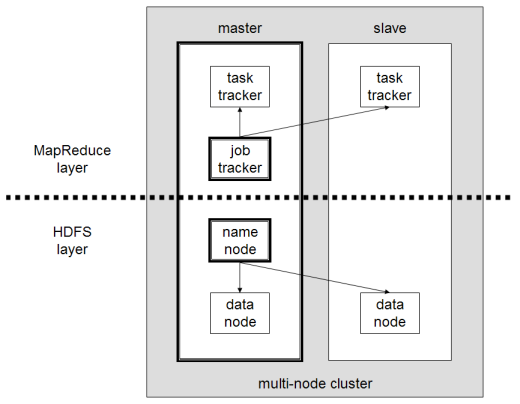
\includegraphics[height=6cm]{img/hadoop-architecture.png}
    \end{center}
  \end{block}
\end{frame}

\begin{frame}{Terms}
  \begin{block}{Hadoop Distributed File System (HDFS)}
    \begin{itemize}
      \item Designed to run on low-cost hardware. 
      \item Computation distribution is more effective than data distribution.
      \item Fault tolerant (data replication).
      \item Batch processing / streaming access.
      \item Large data sets.
      \item NameNode (metadata) for each cluster.
      \item Data nodes $\rightarrow$ racks $\rightarrow$ cluster.
      \item Hundreds of nodes in a single cluster.
    \end{itemize}
  \end{block}
\end{frame}

\begin{frame}{Terms}
  \begin{block}{HDFS}
    \begin{itemize}
      \item DEMO. 
    \end{itemize}
  \end{block}
\end{frame}

\begin{frame}{Terms}
  \begin{block}{MapReduce I}
    \begin{itemize}
      \item Programming model for big data (TBs) parallel processing.
      \item Input data are processed by map-tasks.
      \item Results are combined by reduce-tasks.
      \item Scheduling, monitoring.
      \item Single JobTracker, multiple TaskTrackers.
      \item Client submits a job (jar) and configuration to JobTracker.
      \item (MapR is a company that provides a Hadoop distribution).
    \end{itemize}
  \end{block}
\end{frame}

\begin{frame}{Terms}
  \begin{block}{MapReduce II}
    \begin{center}
      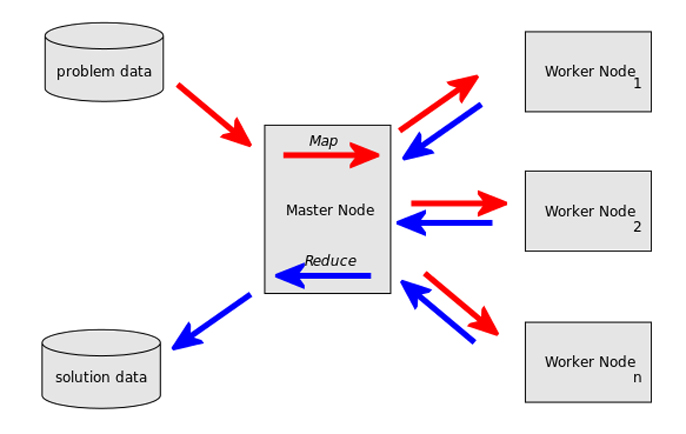
\includegraphics[height=6cm]{img/map-reduce-1.jpg}
    \end{center}
  \end{block}
\end{frame}

\begin{frame}{Terms}
  \begin{block}{MapReduce III}
    \begin{center}
      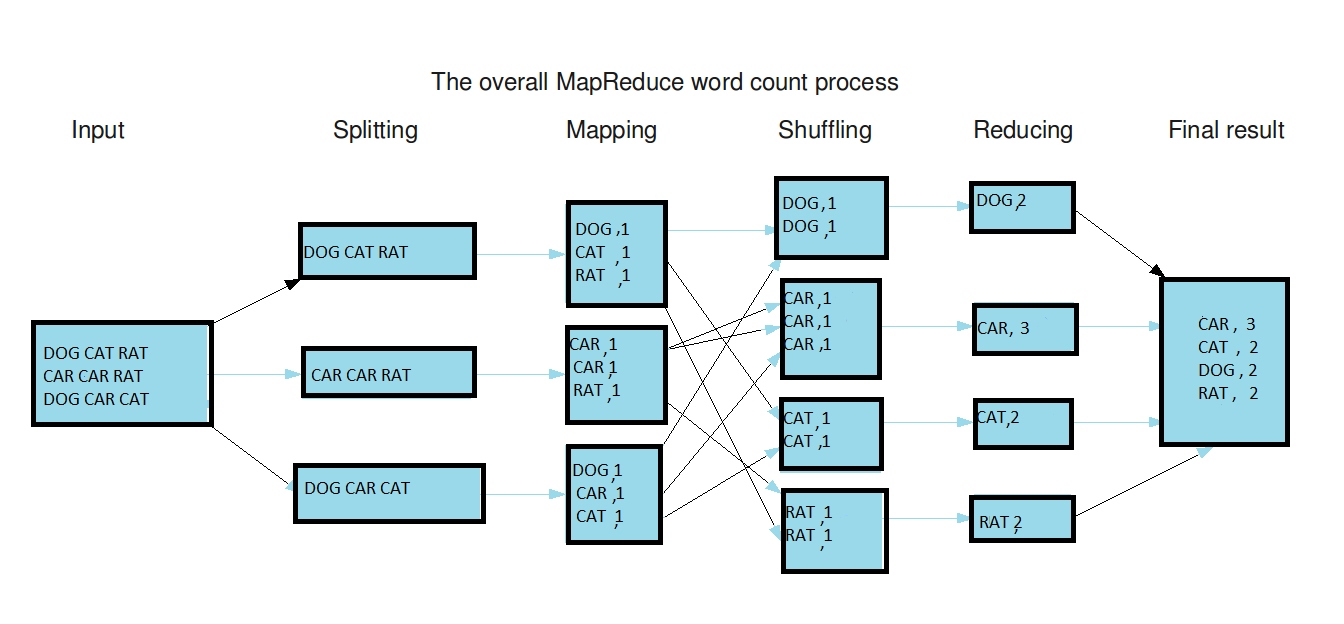
\includegraphics[height=5cm]{img/map-reduce-2.png}
    \end{center}
  \end{block}
\end{frame}

\begin{frame}{Terms}
  \begin{block}{YARN (Yet Another Resource Negotiator)}
    \begin{itemize}
      \item Operating system for big data apps.
      \item Multi tenancy (parallel jobs).
      \item Resource management.
      \item Hadoop2 (MapReduce2).
      \item Decouples resource management from scheduling.
    \end{itemize}
  \end{block}
\end{frame}

\begin{frame}{Terms}
  \begin{block}{YARN Scheduler and Application Managers}
    \begin{center}
      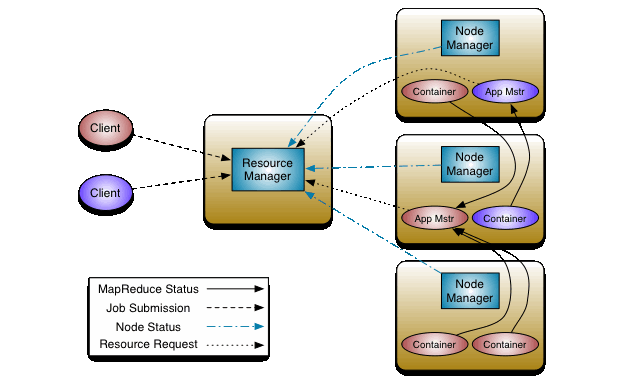
\includegraphics[height=5cm]{img/yarn.png}
    \end{center}
  \end{block}
\end{frame}

\begin{frame}{Terms}
  \begin{block}{Mesos}
    \begin{itemize}
      \item Cross-platform kernel for distributed systems (clusters).
      \item Provides API.
      \item Resource management (CPU, RAM, \dots).
      \item Scheduling.
    \end{itemize}
  \end{block}
\end{frame}

\begin{frame}{Terms}
  \begin{block}{Mesos architecture}
    \begin{center}
      % MPI = message passing interface
      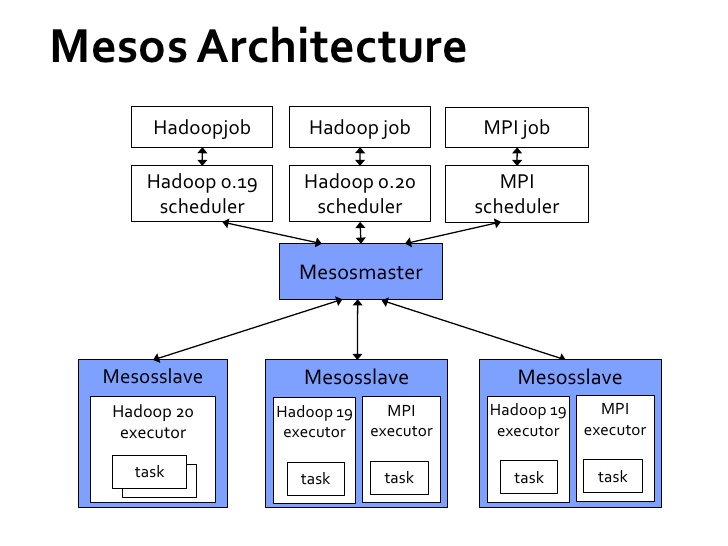
\includegraphics[height=5cm]{img/mesos.jpg}
    \end{center}
  \end{block}
\end{frame}

\begin{frame}{Terms}
  \begin{block}{YARN vs. Mesos}
    \begin{itemize}
      \item They can run parallelly next to each other. 
      \item Main difference is a scheduler.
    \end{itemize}
  \end{block}
  \begin{block}{Hadoop YARN}
    \begin{itemize}
      \item Improvement (next version) of MapReduce API. 
      \item Best suited for Hadoop jobs.
      \item Job request $\rightarrow$ resource manager $\rightarrow$ evaluation $\rightarrow$ assignment.
      \item Server decides.
    \end{itemize}
  \end{block}
  \begin{block}{Apache Mesos}
    \begin{itemize}
      \item Global resource manager (entire data center).
      \item Job request $\rightarrow$ master $\rightarrow$ offers $\rightarrow$ acceptance.
      \item Better scaling capabilities.
      \item Client decides.
    \end{itemize}
  \end{block}
\end{frame}

\begin{frame}{Terms}
  \begin{block}{Spark}
    \begin{itemize}
      \item Open source cluster computing framework.
      \item Data structure oriented API.
      \item RDD (Resilient Distributed Dataset).
      \item Transformations and Actions.
      \item Shared memory.
      \item Database-style querying.
      \item Machine-learning algorithms.
      \item Requires a cluster manager (Spark cluster, YARN, Mesos).
      \item Requires a distributed storage system (HDFS, MapR-FS, Cassandra, \dots).
    \end{itemize}
  \end{block}
\end{frame}

\begin{frame}{Terms}
  \begin{block}{Spark parts}
    \begin{outline}
      \1 Spark Core.
        \2 Tasks, scheduling, I/O, lazy-evaluated RDDs.
        \2 Java, Python, Scala, R.
      \1 Spark SQL.
        \2 DataFrames abstraction layer.
        \2 Structured and semi-structured data.
      \1 Streaming.
        \2 Analytics on mini-batches.
        \2 Support: Kafka, Flume, Twitter, TCP/IP sockets, \dots
      \1 Mlib.
        \2 Statistics, sampling, data generation, classification, \dots
        \2 Cluster analysis methods (k-means).
      \1 Graphx. 
        \2 Graph (edges, vertices) processing framework.
        \2 Based on RDD.
    \end{outline}
  \end{block}
\end{frame}

\begin{frame}{Terms}
  \begin{block}{Spark with DataCleaner}
    \begin{itemize}
      \item DEMO. 
    \end{itemize}
  \end{block}
\end{frame}

\begin{frame}{Terms}
  \begin{block}{Flume}
    \begin{itemize}
      \item Log data collecting tool.
      \item Streaming.
    \end{itemize}
  \end{block}
  \begin{block}{Flume architecture}
    \begin{center}
      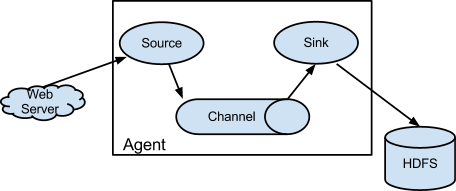
\includegraphics[height=3cm]{img/flume.png}
    \end{center}
  \end{block}
\end{frame}

\begin{frame}{Terms}
  \begin{block}{Flume}
    \begin{itemize}
      \item DEMO. 
    \end{itemize}
  \end{block}
\end{frame}

\begin{frame}{Terms}
  \begin{block}{Sqoop}
    \begin{itemize}
      \item Data transfer between Hadoop and relational database.
      \item CLI tool.
      \item Import: Hive, HBase.
      \item Export: Hadoop $\rightarrow$ relational DB.
    \end{itemize}
  \end{block}
\end{frame}

\begin{frame}{Terms}
  \begin{block}{Sqoop}
    \begin{itemize}
      \item DEMO.
    \end{itemize}
  \end{block}
\end{frame}

\begin{frame}{Terms}
  \begin{block}{HBase}
    \begin{itemize}
      \item Hadoop database.
      \item Non-relational big-data store.
      \item Key-value.
      \item Real-time access.
      \item No sql-scripting.
      \item Java API.
    \end{itemize}
  \end{block}
\end{frame}

\begin{frame}{Terms}
  \begin{block}{Hive}
    \begin{itemize}
      \item Data warehouse.
      \item Sumarization.
      \item Queries.
      \item Analysis.
      \item SQL-like interface (HiveQL).
      \item Command line tool.
      \item Java API.
    \end{itemize}
  \end{block}
\end{frame}

\begin{frame}{Terms}
  \begin{block}{Hive}
    \begin{itemize}
      \item DEMO.
    \end{itemize}
  \end{block}
\end{frame}

\begin{frame}{Terms}
  \begin{block}{Pig}
    \begin{itemize}
      \item Large datasets analyzing platform.
      \item Language Pig Latin.
    \end{itemize}
  \end{block}
\end{frame}

\begin{frame}{Terms}
  \begin{block}{Pig}
    \begin{center}
      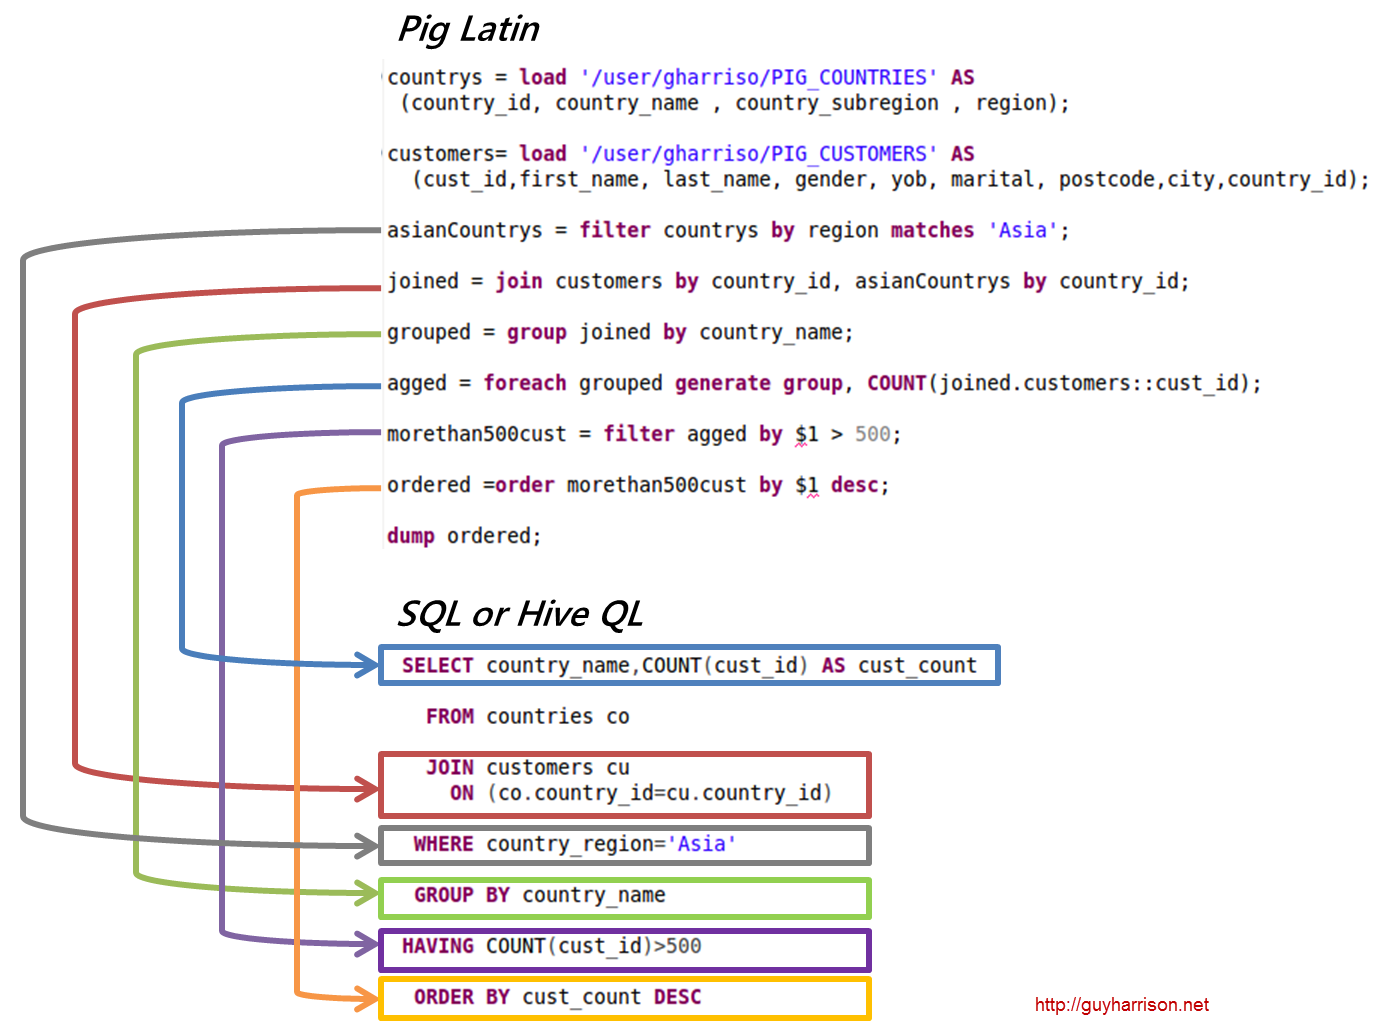
\includegraphics[height=6cm]{img/pig.png}
    \end{center}
  \end{block}
\end{frame}

\begin{frame}{Terms}
  \begin{block}{Oozie}
    \begin{itemize}
      \item Workflow scheduler system.
      \item Triggered by time, frequency or data availability.
      \item Jobs (DAG of actions).
      \item XML.
    \end{itemize}
  \end{block}
\end{frame}

\begin{frame}{Terms}
  \begin{block}{Hue}
    \begin{itemize}
      \item Web interface. 
      \item SQL editor for Hive.
      \item Searching.
      \item Spark and Hadoop notebooks.
      \item Job scheduling (Oozie).
    \end{itemize}
  \end{block}
\end{frame}

